\begin{figure}[H]
    \centering
    \caption{Número de estudos publicados por ano}
    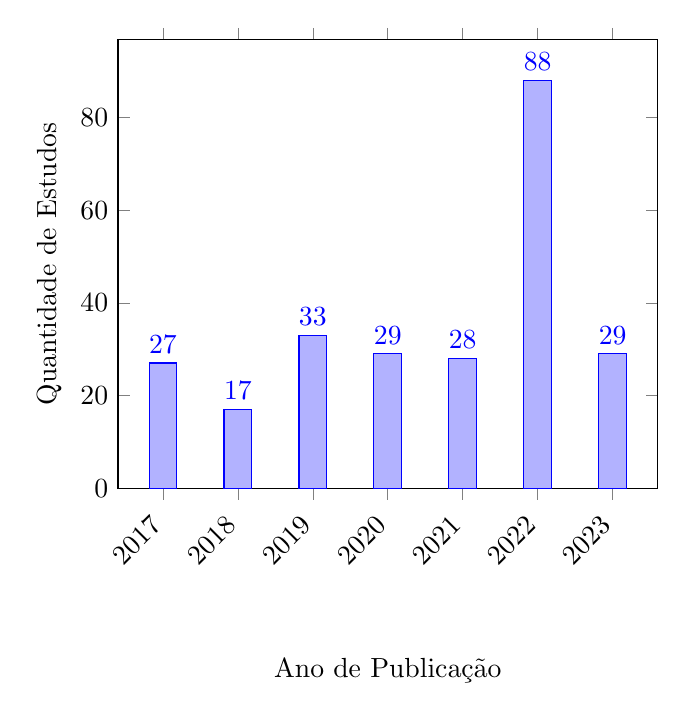
\begin{tikzpicture}
        \begin{axis}[
            ybar,
            symbolic x coords={2017, 2018, 2019, 2020, 2021, 2022, 2023},
            xtick=data,
            ymin=0,
            ylabel={Quantidade de Estudos},
            xlabel={Ano de Publicação},
            xlabel style={yshift=-25pt}, % Move o rótulo do eixo X para baixo
            nodes near coords,
            bar width=10pt, % Aumenta a largura das barras
            enlarge x limits=0.1, % Aumenta o espaçamento entre as barras
            xticklabel style={yshift=-5pt, rotate=45, anchor=east} % Rotaciona e desloca os rótulos do eixo X
        ]
        \addplot coordinates {(2017,27) (2018,17) (2019,33) (2020,29) (2021,28) (2022,88) (2023,29)};
        \end{axis}
    \end{tikzpicture}
    \\
        \centering Fonte: O autor (2024).
\end{figure}
